% \documentclass[round,numbers]{article}  % or book, report, etc.

\documentclass[a4paper,12pt, numbers]{article}

% Import the deliverable package from common directory
\usepackage{../common/deliverable}


% Tell LaTeX where to find graphics files
% \graphicspath{{../common/logos/}{./figures/}{../}}
\graphicspath{{common/logos/}{./figures/}{../}}


\usepackage{xspace}
\usepackage{lipsum}
\usepackage{booktabs}
\usepackage{array}

\newcommand{\dealii}{\texttt{deal.II}}

% Set the deliverable number (without the D prefix, it's added automatically)
\setdeliverableNumber{5.3}

% Begin document
\begin{document}
	
	% Create the title page with the title as argument
	\maketitlepage{Progress report M22}
	
	\newpage
	
	% Main Table using the new environment and command
	\begin{deliverableTable}
		\tableEntry{Deliverable title}{Progress report M22}
		\tableEntry{Deliverable number}{D5.3}
		\tableEntry{Deliverable version}{1.0}
		\tableEntry{Date of delivery}{31 July 2026}
		\tableEntry{Actual date of delivery}{31 July 2026}
		\tableEntry{Nature of deliverable}{Report}
		\tableEntry{Dissemination level}{Public}
		\tableEntry{Work Package}{WP5}
		\tableEntry{Partner responsible}{RUB}
	\end{deliverableTable}
	
	% Abstract and Keywords Section
	\begin{deliverableTable}
		\tableEntry{Abstract}{This report summarizes the project progress in M13--M22, highlighting advances in scalable numerical methods, multiphysics biomedical applications, and exascale computing, as well as key outcomes in project management, communication, and exploitation activities.}
		\tableEntry{Keywords}{progress report; exascale computing; finite element method; biomedical simulations;  management; dissemination; exploitation}
	\end{deliverableTable}
	
	\newpage
	
	\begin{documentControl}
		\addVersion{0.1}{25.07.2026}{Ivan Prusak}{Initial draft}
		\addVersion{0.2}{28.07.2026}{Ivan Prusak}{Techical WP summary}
		\addVersion{0.3}{29.07.2026}{Ivan Prusak}{Non--technical WP summary}
		\addVersion{0.4}{30.07.2026}{Ivan Prusak}{RP1 project review integration}
		\addVersion{0.5}{31.07.2026}{Ivan Prusak}{Update partner contributions}
		\addVersion{0.6}{31.07.2026}{Ivan Prusak}{Deliverable and Milestone status}
		\addVersion{1.0}{31.07.2026}{Martin Kronbichler}{Final version}
	\end{documentControl}
	
	\subsection*{{Approval Details}}
	Approved by: Martin Kronbichler \\
	Approval Date: 31 July 2026
	
	\subsection*{{Distribution List}}
	\begin{itemize}
		\item [] - Project Coordinators (PCs)
		\item [] - Work Package Leaders (WPLs)
		\item [] - Steering Committee (SC)
		\item [] - European Commission (EC)
	\end{itemize}
	
	\vspace*{2cm}
	
	\disclaimer
	
	\newpage
	
	\tableofcontents % Automatically generated and hyperlinked Table of Contents
	
	\newpage
	
	\section{{Introduction}}
	
	
	\subsection{Purpose of the Document}
	
	This document provides an overview of the dealii-X project activities, achievements, and challenges during the reporting period M13–M22. Its main purpose is to give a clear and comprehensive account of the work carried out, highlighting both scientific and technical progress as well as management, communication, and exploitation efforts. 
	
	The report covers progress in developing an exascale framework for digital twins of the human body. It details advances in scalable numerical methods, high-perfor\-mance computing strategies, and multiphysics biomedical applications. These technical developments are accompanied by efforts to ensure the reliability, efficiency, and usability of the software, which form the foundation for future scientific and clinical applications.
	
	In addition to the scientific and technical aspects, this document also reports on project management, communication, and exploitation activities. This includes coordination between partners, dissemination of results to the wider scientific community, and strategies to promote uptake and impact of the outputs of the project. By integrating these different dimensions, the report not only documents achievements but also provides context for planning the next steps and setting priorities for the upcoming phases of the project.
	
	Overall, this report serves as both a record of past activities and a guide for future work, helping to maintain transparency, accountability, and alignment with the overarching project goals.
	
	
	\subsection{{Structure of the Document}}
	\begin{itemize}
		\item Section \ref{sec:wp1_dealii}: dealii-X exascale building blocks and support tools (WP1)
		\item Section \ref{sec:wp2_applications}: dealii-X lighthouse Applications for Digital Twins of the Human Body (WP2)
		\item Section \ref{sec:wp3_codesign}: Co-Design, Technology Exploitation, and Energy Efficiency (WP3)
		\item Section \ref{sec:wp4_communication}: Dissemination, Communication, and Exploitation (WP4)
		\item Section \ref{sec:wp5_management}: Project Management (WP5)
	\end{itemize}
	
	\newpage
	
	\section{{dealii-X exascale building blocks and support tools (WP1)}}
	\label{sec:wp1_dealii}
	
	\subsection{Objectives}
	
	The main objective of Work Package 1 (WP1) is to serve as the foundation
	for the dealii-X Centre of Excellence by enhancing and expanding the
	capabilities of the deal.II finite element library to address the challenges of exascale
	computing and facilitate the creation of advanced digital twins of human
	organs.
	
	The key steps of WP1 include:
	\begin{itemize}
		\item extending and improving the exascale capabilities for the main
		algorithmic kernels of \dealii;
		\item improving pre-exascale modules of the \dealii{} library;
		\item developing an experimental polygonal discretization module for \dealii;
		\item integrating PSCToolkit within \dealii{};
		\item integrating MUMPS within \dealii{}.
	\end{itemize}
	
	Specifically, the sub-work packages aim to:
	\begin{itemize}
		\item \textbf{WP1.1 (Lead RUB)}: Develop matrix-free algorithms for GPU
		architectures and enhance \dealii's performance on exascale systems; design and implement scalable algorithms for multiphysics problems; optimize performance and enhance scalability of matrix--free and matrix--based solvers in \dealii{} for large-scale EuroHPC systems;  
		\item \textbf{WP1.2 (Lead UNIPI)}: Improve the gmsh API, develop a generalized interface for coupling operators in \dealii{}, enhance \dealii's reduced order modeling capabilities, integrate low-rank approximation methods, and develop block preconditioners for coupled problems;
		\item \textbf{WP1.3 (Lead SISSA)}: Introduce and enable polygonal discretization methods within \dealii{} at large scale;  develop methods for construction of coarse grid hierarchies and agglomeration--based multigrid techniques; explore the use of polygonal discretization methods as preconditioners for multiphysics problems;
		\item \textbf{WP1.4 (Lead UNITOV)}: integrate PSCToolkit into deal.II, utilize GPU computing with integrated framework; develop and implement efficient preconditioners for multiphysics problems;
		\item \textbf{WP1.5 (Lead INPT)}: integrate the MUMPS solver directly into \dealii{} for use in multigrid and domain decomposition methods; utilize MUMPS as a coarse grid solver in multigrid methods implemented in PSCToolkit; optimize MUMPS for use with GPU systems; explore low-rank and mixed-precision techniques to improve computational efficiency.
	\end{itemize}
	
	In summary, WP1 is dedicated to developing and integrating advanced algorithms and fundamental software components within the \dealii{} library and external libraries, with a strong emphasis on enabling exascale compute capabilities for the digital twin applications in WP2.
	%(M1–M12)
	
	
	\subsection{WP1.1: Extending and improving the exascale capabilities in deal.II} % (M1–M22, Lead: RUB)}

Work package WP1.1 focuses on enabling efficient finite element computations
with the deal.II finite element library, where matrix-free evaluation
techniques and multigrid methods are the core scientific components.

The activities of the group at RUB can be summarized as follows:
\begin{itemize}
	% \item Extension of matrix-free implementations for modern GPUs in deal.II, including testing and performance evaluation through CEED benchmarks.
	\item node--level optimization and benchmarking of the high--order matrix--free kernels and solvers,
	\item extension of the GPU--ready kernels to various discretization techniques in \dealii,  
	\item developing portable multigrid solvers and multigrid infrastructure in \dealii,
	\item scalability of single-physics solvers to large node counts on EuroHPC systems.
\end{itemize}



\subsubsection*{Performance Evaluations of High Order Finite Element Kernels on Modern Accelerators}

\noindent Recent enhancements to the \texttt{dealii-X} matrix-free framework encompass architectural optimizations and performance benchmarks across NVIDIA, AMD, and Intel platforms.

\noindent\textbf{Kernel enhancements and optimizations.}
The Kokkos-based CEED\footnote{\url{https://ceed.exascaleproject.org/bps}, retrieved on 28.07.2026} bake-off kernels within the \texttt{dealii-X} benchmark repository\footnote{\url{https://github.com/dealii-x/benchmarks}, retrieved on 28.07.2026} have been expanded using two- and three-dimensional thread structures to maximize thread-wise data locality and hardware throughput. The usage of  C++ templates allowed for significant compile-time optimizations, including loop unrolling. To mitigate streaming multiprocessor (SM) and wavefront underutilization observed for low polynomial orders ($p=1, 2$), the implementation transitioned from a single-element-per-block model to a batched multi-element processing strategy (e.g., fitting up to 11 elements per thread block for BK3 $p=1$). 

\noindent\textbf{Performance highlights and key results.}
On the NVIDIA GH200 Grace Hopper Superchip, the Kokkos-based Stream Triad benchmark established an effective reference memory bandwidth of $3.65\text{ TB/s}$. Across evaluated GPU architectures, the AMD MI210 nearly doubled the throughput compared to the Intel Max 1550, despite similar bandwidth figures ($\sim 1.25\text{ TB/s}$ vs.\ $1.0\text{ TB/s}$). Peak single-precision (FP32) throughputs on the GH200 reached nearly $90\text{ GDOF/s}$ for BK1 and BK5, while BK3 plateaued at approximately $25\text{ GDOF/s}$. Critically, the new batched processing technique yielded a $2\times$ speedup for $p=1$ on the NVIDIA GH200 (JUPITER supercomputer). The results are documented in the reports for Deliverables D1.7, D1.9, D3.3 and D3.4.

\noindent\textbf{CEED benchmark Problems.}
The operator evaluation framework was further extended to a complete linear solver by embedding the Laplace operator within a Conjugate Gradient (CG) method, corresponding to the CEED Bake-Off Problem (BP) benchmarks. Implemented within \dealii{}, the solver was evaluated on single- and multi-GPU configurations of the GH200 Superchip using MPI with peer-to-peer (P2P) communication enabled. Results indicate that performance differences between standalone operator evaluations (BK) and full solvers (BP) are primarily driven by gather-scatter overheads and inter-GPU communication. Additionally, the evaluations confirm the high computational efficiency of high-order elements, which leverage tensor-product formulations of shape functions to increase arithmetic intensity. The results are documented in the reports for Deliverables D1.7, D1.9, D3.3 and D3.4.


\subsubsection*{New matrix--free kernels for various finite elements.}

Recent developments expand the matrix-free evaluation capabilities to $H(\text{div})$--confor\-ming Raviart--Thomas spaces and Discontinuous Galerkin (DG) formulations across modern accelerator platforms.

\noindent\textbf{Raviart--Thomas elements and tensor core integration.}
Matrix-free kernels for the core operators of $H(\text{div})$--conforming Raviart--Thomas elements---vector mass, mixed divergence, and mixed gradient---were implemented and benchmarked. On the NVIDIA GH200 (JUPITER), batch processing yields consistent throughput across polynomial orders in both FP32 and FP64 precision. Similar high throughput is observed on the AMD MI250X GPU (LUMI supercomputer), with a performance drop restricted to $p=8$ due to register file capacity constraints. Furthermore, target support for NVIDIA Tensor Cores was introduced for FP64 and non-IEEE-compliant TensorFloat-32 (TF32) matrix multiplications. The results are documented in the reports for Deliverables D1.9 and D3.4.

\noindent\textbf{Discontinuous Galerkin kernels.}
Matrix-free Discontinuous Galerkin (DG) face integration was developed for symmetric interior penalty (Nitsche) discretizations of the Laplace operator, handling both cell volume terms and numerical flux integrals over face interfaces via average and directed jump operators. Initial evaluations employ a face-centric loop (FCL) algorithm with global temporary storage to process face interactions across adjacent cells. Current efforts focus on communication reduction and cell-centric face integration paradigms ahead of a comprehensive scalability study. The preliminary results are reported in Deliverable D1.9. 

\subsubsection*{Portable Multigrid Framework}

\noindent Matrix-free algorithms were integrated into the capable multigrid infrastructure of \dealii{}, featuring GPU-accelerated polynomial and geometric transfer operators using Kokkos abstractions and device-aware MPI.

\noindent\textbf{Portable multigrid infrastructure.}  Incorporating the matrix--free kernel developments, an extensive multigrid infrastructure covering both geometric and polynomial variants has been developed within the \texttt{dealii-X portable-multigrid} repository.\footnote{\url{https://github.com/dealii-X/portable-multigrid}, retrieved on 28.07.2026} Core matrix-free geometric transfer functionality has been integrated upstream into \dealii{} and included in \dealii{} upcoming release 9.8. The infrastructure was ported to the JUPITER supercomputer at the Jülich Supercomputing Centre (JSC), leveraging both Nvidia Grace CPU Neon vectorization and Hopper GPU capabilities within the GH200 Superchip. 

\noindent\textbf{Mixed--precision strategies.}
Combining a single-precision (FP32) multigrid V-cycle preconditioner with an outer double-precision (FP64) conjugate gradient solver demonstrated superior performance and robustness compared to pure FP64 implementations. Matrix-vector evaluations on continuous finite elements established high single-GPU throughput across broad problem sizes. The preliminary results are reported in Deliverables D1.7 and D1.9.

\noindent\textbf{Performance and weak scaling benchmarks.}
Weak scaling results (reported in Deliverable D1.7) on up to 128 nodes (512 GPUs) of JUPITER, using $57$--$65$ million unknowns per GPU, showed very good matrix-vector product scaling with approximately 65\% parallel efficiency. However, overall multigrid efficiency degraded significantly across scale, with runtime increasing by a factor of $2.5$ over a $128\times$ size increase despite algorithmic optimality. This behavior was traced to communication latency on the coarser levels of the multigrid hierarchy, where fixed ghost-exchange overheads ($\ge 7 \times 10^{-4}\text{ s}$ per step) for smaller message sizes. Following the recommendation of the intermediate review, the service of the POP3 (Performance Optimisation and Productivity) Centre of Excellence has been secured, and the analysis report is expected by September 2026. Additionally, a researcher with extensive experience in MPI and communication--avoiding strategies has joined the project for its remaining duration.

\noindent\textbf{Extension to DG multigrid solvers.}
The framework was further extended to Discontinuous Galerkin (DG) discretizations, incorporating a mixed-precision $cph$--multi\-grid solver that embeds the discontinuous space into a continuous space at the finest level. Throughput evaluations show that DG elements reach a distinct performance plateau that scales consistently across increasing GPU counts. Unlike Continuous Galerkin (CG) operators, which exhibit very strong latency effects, DG face integration demonstrates strong multi-GPU scaling potential as reported in Deliverable D1.9.



\subsection{WP1.2: Improvement of pre-exascale modules of the deal.II library} % (M1–M22, Lead: UNIPI)}

Work package 1.2 focuses on enhancing the existing modules of the deal.II library to prepare them for the challenges of exascale computing.  

The overall objective is to improve the pre-exascale functionalities of deal.II,
making it an even more robust and efficient library for a wide range of
scientific and engineering applications aiming for the use of exascale
computers.

\subsubsection*{VTK Interoperability and Data-Ingestion Utilities}

\noindent Robust data-ingestion utilities have been established to enable seamless interoperability between external scientific computing pipelines and the \texttt{dealii-X} framework via native Visualization Toolkit (VTK) APIs.

\noindent\textbf{VTK integration and data flow.}
Capabilities to import VTK meshes alongside point and cell fields using native VTK APIs, as well as bi-directional conversion between VTK unstructured grids and \dealii{} triangulations, have been implemented. This direct VTK API usage facilitates streamlined integration with external pre--processing tools, enables reproducible mesh and field reuse for surrogate modeling, and minimizes custom glue code across lighthouse applications. The VTK utilities workstream is coordinated under meta-issue \#19056.\footnote{\url{https://github.com/dealii/dealii/issues/19056}, retrieved on 28.07.2026}

\subsubsection*{New Tutorials under the \texttt{dealii-X} Label}

\noindent A new tutorial framework implementing a fully coupled fluid--structure interaction (FSI) solver was developed to provide a realistic benchmark for advanced linear solvers and multiphysics workloads.

\noindent\textbf{Immersed boundary FSI formulation.}
The tutorial demonstrates a finite element immersed boundary method with distributed Lagrange multipliers for fully coupled FSI. An incompressible fluid governed by Navier--Stokes equations is coupled to a compressible, hyper-elastic solid on independent, non-matching volumetric meshes. Velocity continuity across interfaces is enforced via a multiplier field $\lambda$ rather than penalization, combining particle-based transfer, \texttt{MappingFEField}-driven solid motion, and a monolithic saddle-point solve for four--component fluid--structure-multiplier field. This framework directly targets coupled multiphysics applications such as cardiovascular flows, brain mechanics, and lung/liver mechanics.

\noindent\textbf{Preconditioning milestone completion.}
The implementation showcases an augmented Lagrangian preconditioner designed to handle the coupled saddle-point structure, providing a realistic test bench for linear solver capabilities developed within \texttt{dealii-X}, including PSCToolkit-based preconditioning and advanced MUMPS configurations. Together, these developments mark the completion of Milestone \#7: \emph{Scalable Coupling Algorithms Framework Completion}.

\subsubsection*{Hybridizable Discontinuous Galerkin Solver for Vascular Networks}

\noindent An implicit Hybridizable Discontinuous Galerkin (HDG) framework was developed within \dealii{} to simulate reduced-order one-dimensional blood flow in complex arterial networks.

\noindent\textbf{Governing formulation and HDG discretization.}
The formulation models non-linear conservation laws for cross-sectional area and mean velocity parameterized along network centerlines, incorporating non-linear physical flux terms, viscous friction, and a non-linear tube law for arterial wall elasticity. The spatial discretization employs an HDG scheme utilizing the Harten--Lax--van Leer (HLL) numerical flux alongside a unified trace formulation to enforce interface continuity across interior boundaries, physiological outlets (single-resistance and three-element Windkessel RCR models), and multi-vessel vascular junctions (including bifurcations).

\noindent\textbf{Time integration and monolithic solver.}
The semi-discrete HDG system was integrated with the \textsc{SUNDIALS} IDA solver for fully implicit time integration. A monolithic Newton framework was constructed using analytical Jacobians and full residual assembly, eliminating the necessity for sub-Newton iterations within each global step.

\noindent\textbf{Validation and mesh convergence.}
Validation was conducted on the 37-artery human systemic network benchmark, consisting of 37 arterial segments connected through 21 bifurcations driven by a physiological inflow waveform. Comparisons of pressure, flow rate, and cross-sectional area at the thoracic aorta II against established finite-volume benchmarks demonstrated excellent agreement across the cardiac cycle. Successive mesh refinement studies confirmed spatial mesh independence and rapid solution convergence. The results are reported in Deliverable D1.9.


\subsection{WP1.3: Experimental polygonal discretization module for deal.II} % (M1–M22, Lead: SISSA)}
The primary objective of this sub work package is the development of a polygonal
discretization module within the deal.II library. The deal.II library currently
supports a wide range of finite element methods, defined on standard simplicial
and hexahedral meshes, but does not support polygonal and polyhedral (\emph{polytopic}) meshes.

\subsubsection*{Polygonal Discretization Module}

\noindent The polygonal discretization activity integrates general-mesh capabilities into the \dealii{} library, focusing on discontinuous Galerkin methods on agglomerated polygonal/polyhedral meshes and automatic coarse grid hierarchy construction.

\noindent\textbf{Polydeal library.}
The supporting library, \texttt{Polydeal},\footnote{\url{https://github.com/fdrmrc/Polydeal}, retrieved on 28.07.2026} provides the computational foundation for agglomerated polytopic discretizations. It is continuously updated to align with the latest version of \dealii{}, strictly adhering to its coding style, design practices, and quality standards. Comprehensive continuous integration test suites are executed on every commit to ensure long-term codebase integrity and stability.

\noindent\textbf{Code Gallery tutorial.}
To showcase practical applications, a self-contained tutorial program demonstrating an agglomeration-based Poisson solver was submitted to the \dealii{} Code Gallery via pull request \#233.\footnote{\url{https://github.com/dealii/code-gallery/pull/233}, retrieved on 28.07.2026} Following review and approval, the \texttt{agglomeration\_poisson} tutorial, complete with documentation and numerical results, was published on the official \dealii{} Code Gallery page,\footnote{\url{https://dealii.org/developer/doxygen/deal.II/code_gallery_agglomeration_poisson.html}, retrieved on 28.07.2026} supplemented by layout rendering enhancements in pull request \#244.\footnote{\url{https://github.com/dealii/code-gallery/pull/244}, retrieved on 28.07.2026}

\noindent\textbf{Integration in deal.II.}
Core reusable components from \texttt{Polydeal} were separated from application code, adapted to native \dealii{} conventions, and submitted to the main core repository via pull request \#19891.\footnote{\url{https://github.com/dealii/dealii/pull/19891}, retrieved on 28.07.2026} This contribution establishes a framework for DG discretizations on agglomerated meshes, introducing agglomeration management, standard accessor/iterator interfaces, degree-of-freedom and sparsity-pattern construction, agglomeration-aware mapping and quadrature, and R-tree-based hierarchical agglomeration (detailed in the report for Deliverable D1.8).

\subsubsection*{Geometrically Informed Multilevel Preconditioning}

\noindent A geometrically informed algebraic multigrid preconditioner was developed for discontinuous Galerkin (DG) discretizations of elliptic problems on complex, fine unstructured geometries.

\noindent\textbf{Agglomeration-based multigrid strategies.}
Leveraging the mesh agglomeration functionality within \texttt{Polydeal}, a hierarchy of nested agglomerated coarse polytopal grids is constructed from fine unstructured meshes. Coarse grid operators are constructed either by rediscretizing the PDE on agglomerated meshes or via triple Galerkin projections without rediscretization. The finest level retains a hexahedral structure, enabling the exploitation of tensor-product basis functions and matrix-free operator evaluation within \dealii{}.

\noindent\textbf{Application to cardiac electrophysiology.}
The multigrid scheme was applied as a V-cycle preconditioner within a preconditioned conjugate gradient (PCG) solver for the DG discretization of the cardiac electrophysiology monodomain model across high-order polynomial degrees ($p=1, 2$) on a realistic 3D ventricular mesh. Benchmarks against Trilinos ML algebraic multigrid (AMG) demonstrated lower PCG iteration counts and significant reductions in wall-clock time per iteration. Ongoing research aims to integrate this approach into established AMG frameworks and construct matrix-free implementations for coarse operators. The results are reported in Deliverable D1.7.

\subsubsection*{Unfitted Space--Time DG Method on Moving Domains}

\noindent Theoretical developments extend the general-mesh DG philosophy to parabolic problems posed on time-dependent physical domains embedded within fixed background space--time meshes.

\noindent\textbf{Space--time agglomeration strategy.}
The evolving physical domain is tracked via a time-dependent level-set function on a fixed background mesh, avoiding full-domain remeshing at each time step. To eliminate small-cut cell instabilities, background elements with minimal domain intersections are agglomerated with neighboring elements, yielding robust polytopic space--time elements that satisfy uniform geometric bounds independent of the cut configuration. More details are available in Deliverable D1.9.

\noindent\textbf{Formulation and theoretical stability.}
A space--time DG formulation was established on the agglomerated space--time mesh. Theoretical analysis verified coercivity and inf-sup stability estimates that remain uniform relative to the moving boundary position, alongside optimal a priori error bounds in a DG energy norm controlling the broken $H^1$-seminorm. More details are available in Deliverable D1.9.

\subsection{WP1.4: Integration of PSCToolkit within deal.II} \label{sec:wp1_psctoolkit}% (M1–M22, Lead: UNITOV)}

Work package 1.4 integrates the Parallel Sparse Computing Toolkit (PSCToolkit) into \dealii{}, with the objective of providing scalable algebraic multigrid (AMG) preconditioning through the AMG4PSBLAS package as a drop-in replacement for the existing AMG interfaces.

\subsubsection*{Integration status}

\noindent\textbf{Linear algebra backbone.}
The integration has advanced to a mature stage during this reporting period. The numerical linear algebra backbone provided by the PSBLAS library is now fully integrated into the \dealii{} main repository, through pull requests \#18938 and \#19356.\footnote{\url{https://github.com/dealii/dealii/pull/18938} and \url{https://github.com/dealii/dealii/pull/19356}, retrieved on 30.07.2026} The user interface follows the design of the existing \dealii{} linear algebra frameworks: the \texttt{PSCToolkitWrappers} namespace mirrors the structure of the Trilinos and PETSc wrappers, so that switching between AMG implementations requires no structural changes to application code. Unit tests have been added to ensure correctness and to prevent regressions in future developments.

\noindent\textbf{AMG preconditioners.}
The AMG4PSBLAS preconditioners are exposed through the \texttt{PreconditionAMG} class, which builds the multilevel hierarchy from a distributed PSBLAS system matrix and applies it through the standardized \texttt{vmult()} method. Smoother type, coarsening strategy and coarse grid solver are configured through an \texttt{AdditionalData} object, in the same manner as the other \dealii{} preconditioner interfaces. This contribution is under review in pull request \#19398.\footnote{\url{https://github.com/dealii/dealii/pull/19398}, retrieved on 30.07.2026} The interface and its usage are documented in Deliverables D1.6 and D1.7.

\subsubsection*{Performance assessment on MareNostrum 5}

\noindent\textbf{Weak scaling on a model problem.}
Following validation of the interface on the tutorial application documented in Deliverable D1.6, the practical performance of the AMG preconditioners was assessed on the MareNostrum 5 supercomputer at the Barcelona Supercomputing Center. A three-dimensional Poisson problem on the unit cube, discretized with $\mathcal{Q}_1$ elements on a uniform hexahedral mesh, is solved by conjugate gradient preconditioned with a single smoothed V-cycle using parallel matching aggregation (\texttt{MatchBoxP}), a degree-four polynomial smoother and an $\ell_1$-Jacobi coarsest level solver. Weak-scaling runs on 1, 8 and 64 nodes (24 MPI ranks per node), corresponding to approximately $2.15\times 10^{6}$, $1.70\times 10^{7}$ and $1.35\times 10^{8}$ unknowns, keep the cost per CG iteration within a narrow range of $0.08$--$0.10$ s while the operator complexity of the hierarchy remains essentially constant at approximately $2$, indicating that the quality of the AMG hierarchy is preserved as the problem size grows. The results are reported in Deliverable D1.9.

\noindent\textbf{Strong scaling on a realistic cardiac test case.}
The preconditioner was further assessed on the linear system arising from the monodomain model in cardiac electrophysiology, discretized on a fixed, unstructured, patient-specific left ventricle mesh with approximately $2.4\times 10^{7}$ degrees of freedom. With the same preconditioner configuration, the conjugate gradient solver reduces the relative residual by eight orders of magnitude in $12$ iterations, independently of the number of MPI ranks employed, confirming the algorithmic scalability of the aggregation strategy on unstructured, patient-derived geometries. The strong-scaling behaviour is reported in Deliverable D1.9.

\subsubsection*{Ongoing and future work}

\noindent\textbf{GPU support and outlook.}
PSBLAS provides GPU acceleration primarily through CUDA backends, and the exposition of this functionality through the \dealii{} interface has already been implemented, with the corresponding pull request to be submitted shortly. The remaining activities concern larger-scale performance evaluations on EuroHPC systems and the assessment of the AMG preconditioners on coupled multiphysics problems. In collaboration with INPT, the use of Block Low-Rank approximations as smoothers within the AMG cycles is being explored, linking the developments of WP1.4 and WP1.5.
\subsection{WP1.5: Integration of MUMPS within deal.II} % (M1–M22, Lead: INPT)}
WP1.5 aims to integrate the MUMPS (Multifrontal Massively Parallel Sparse) solver directly into deal.II and improve the capabilities of the MUMPS solver. This task focuses on enabling its use in multigrid methods and exploring advanced techniques such as low-rank approximations and mixed-precision computations to enhance solver efficiency.


\subsubsection*{Integration Status}
A direct interface between \dealii{} and MUMPS has been completed and integrated into the \dealii{} main repository, exposing BLR compression and mixed-precision options through the standard solver interface and enabling MUMPS as a coarse grid solver within multigrid and domain decomposition methods. On representative organ simulation benchmarks the integration delivers a $15\times$ reduction in solve time and a $5\times$ reduction in memory consumption relative to the previous configuration, which made full-organ brain indentation problems tractable for the first time.


\subsubsection*{Block Low-Rank (BLR) Approximation}

\noindent Recent advancements in sparse direct solver techniques integrate low-rank approximations and mixed-precision algorithms into the MUMPS library within the \texttt{dealii-X} framework to drastically reduce computational complexity and memory footprint.

\noindent\textbf{Direct solver capabilities.}
Direct solver integration targets high-resolution organ simulation workloads arising in \dealii{}, such as brain indentation benchmarks comprising $2.4\times 10^7$ degrees of freedom and $9 \times 10^5$ elements. Evaluating sparse direct factorizations demonstrates that exploiting data sparsity and low-rank structures mitigates the prohibitive floating-point operation counts and memory overheads traditional full-rank direct solvers face. Recent evaluations across accelerated hardware platforms (NVIDIA Grace Hopper, AMD MI250/MI300) demonstrate $3\times$ to $6\times$ speedups for full-rank factorizations, establishing a foundation for accelerated low-rank integration. The results are reported in Deliverables D1.7, D1.9, D2.3 and D2.4.

\noindent\textbf{Adaptive-precision BLR.}
MUMPS leverages BLR compression to represent dense frontal matrix blocks during numerical factorization, with compression levels controlled by a user-defined threshold $\varepsilon$. Incorporating adaptive precision BLR allows column factors to be stored at varying floating-point precisions based on singular value magnitudes. Benchmarks on 3D organ simulation matrices show LU factor memory reductions of up to $50\%$, peak memory decreases of $26\%$, and operation count (FLOPS) savings up to $85\%$ relative to full-rank factorizations. The results are reported in Deliverables D1.7 and D1.9.

\subsubsection*{Iterative Mixed Precision}

\noindent Mixed-precision algorithms combine multiple floating-point formats to maximize hardware throughput while preserving full target accuracy through iterative refinement.

\noindent\textbf{Mixed LU iterative refinement (LU-IR).}
Mixed-precision LU iterative refinement executes time- and memory-intensive $LU$ factorizations in single precision (FP32) while calculating residual updates in double precision (FP64). Combining FP32 factorization with FP64 iterative refinement recovers full double-precision accuracy while reducing factorization time and memory consumption by roughly $50\%$. When combined with adaptive BLR compression, this mixed-precision strategy achieves an overall $77\%$ reduction in memory footprint and a $63\%$ reduction in total factorization runtime compared to standard double-precision full-rank solvers. The results are reported in Deliverables D1.7 and D1.9
\newpage

\section{{dealii-X lighthouse Applications for Digital Twins of the Human Body (WP2)}}
\label{sec:wp2_applications}


\subsection{Objectives}

The overall objective of WP2 is to advance accurate, efficient, and scalable digital twins of major human organs, building on the algorithmic innovations of WP1. Each sub-workpackage targets a specific domain while contributing to a unified multi-organ framework.

The key applications of WP2 include:
\begin{itemize}
\item Exascale simulations of the respiratory system;
\item Exascale simulations in cardiac computational medicine;
\item Exascale simulations of brain tissue mechanics;
\item Development of a digital twin for the human liver;
\item Development of a digital twin for cellular interactions;
\item Low-code platform for human organ digital twin creation.
\end{itemize}

Specifically, the sub-work packages aim to:
\begin{itemize}
\item \textbf{WP2.1 (Lead TUM)}: Develop exascale-ready solvers for respiratory flow and transport, with advanced time
stepping, mixed meshes, and fluid–structure interaction, extending later to other biomedical flows;
\item \textbf{WP2.2 (Lead POLIMI)}: Enhance the \texttt{lifex} software for exascale cardiac simulations, including GPU-enabled solvers, high-order FEM, multiphysics integration, and multiscale models of healthy and pathological conditions;
\item \textbf{WP2.3 (Lead FAU)}: Optimize an HPC brain solver with parallelization, GPU acceleration, and nonlinear routines, enabling high-fidelity, patient-specific brain simulations;
\item \textbf{WP2.4 (Lead FVB-WIAS)}: Build and validate a liver simulator prototype with enhanced poro-visco-elastic models, realistic geometries, and coupling with cardiovascular flows;
\item \textbf{WP2.5 (Lead UNIBS)}: Develop cell-scale digital twins using novel space–time FEM and coupling of receptor dynamics with flow, validated against in vitro data;
\item \textbf{WP2.6 (Lead EXACT LAB)}: Deliver a low-code platform and meta-scheduler to simplify digital twin construction and execution across HPC resources.
\end{itemize}

Together, the WP2 subprojects aim to push the boundaries of computational simulations for major human organs, leveraging and integrating the advancements in exascale computing and the deal.II software library produced in WP1. Table~\ref{tab:wp1wp2} reports on the  \dealii{} and dealii-X functionalities employed by each lighthouse application.

\begin{table}[htbp]
	\centering
	\caption{\dealii{} and dealii-X functionalities employed by the individual lighthouse applications.}
        \label{tab:wp1wp2}
        \medskip
	\renewcommand{\arraystretch}{1.2}
	\footnotesize
	\begin{tabular}{p{3.0cm}p{11.0cm}}
		\toprule
		\textbf{Application} & \textbf{WP1 functionalities employed} \\
		\midrule
		WP2.1 Lungs & Matrix-free kernels; polynomial multigrid; mixed-precision preconditioning \\
		\midrule
		WP2.2 Heart & Matrix-free evaluation (\texttt{FEEvaluation}); $p$-multigrid with Chebyshev smoothing; block preconditioners; agglomeration-based multigrid for electrophysiology; AMG4PSBLAS (PSCToolkit) preconditioning\footnotemark[1] \\
		\midrule
		WP2.3 Brain & MUMPS direct solver with BLR compression and mixed precision; distributed triangulations \\
		\midrule
		WP2.4 Liver  & Coupling operators for non-matching grids; augmented Lagrangian preconditioners; Gmsh-based mesh generation \\
		\midrule
		WP2.5 Mechanobiology  & Distributed triangulations with independent AMR; non-matching field transfer between bulk and surface meshes \\
		\bottomrule
	\end{tabular}
\end{table}

\footnotetext[1]{AMG4PSBLAS has been assessed on the cardiac electrophysiology monodomain problem on a patient-specific left ventricle mesh (Section~\ref{sec:wp1_psctoolkit}); its integration into the application codes is foreseen in the final project period.}





\subsection{WP2.1 Lungs: Exascale Simulations of the Respiratory System}

\subsubsection*{Surfactant Model for Alveolar Mechanics}

\noindent Recent developments in the ExaDG\footnote{\url{https://github.com/exadg/exadg}, retrieved on 29.07.2026} structural module introduce an enhanced-surface finite element formulation to capture nonlinear, surface-tension-driven mechanics in lung applications.

\noindent\textbf{Surface-tension weak formulation.}
The enhanced-surface model incorporates the time- and frequency-dependent mechanics of surface tension at element boundaries without explicitly resolving fluid-lining layers or surfactant molecules. Weak forms integrate an additional boundary integral of surface tension evaluated as a multivariate function of solution variables and local history data. Integrating this formulation required substantial revisions to boundary integral evaluation routines within ExaDG to support solution-dependent boundary terms.

\noindent\textbf{Verification on idealized alveolar geometries.}
Model verification was conducted using an idealized spherical alveolus. Comparative compliance evaluations demonstrate that while an unlined surface exhibits the highest compliance, physiological function requires a fluid lining for gas exchange. Unlined water films yield the lowest compliance (pathological cases), whereas introducing surfactant molecules significantly reduces surface tension, enhancing alveolar compliance, volume expansion, and displacement dynamics required for efficient gas exchange.

\subsubsection*{Multigrid Solver Performance and Complex Geometries}

\noindent Performance optimizations focused on identifying robust preconditioning strategies for structural solves on quadratic tetrahedral discretizations of complex alveolar networks.

\noindent\textbf{Polynomial multigrid (pMG) evaluation.}
Collaborative solver evaluations identified polynomial multigrid (pMG) as an effective candidate for high-order finite element formulations. Despite initial concerns regarding shear and volumetric locking on coarse linear tetrahedral elements, pMG with algebraic multigrid (AMG) coarse solver demonstrated superior iteration counts and runtime performance over pure AMG on bending beam benchmarks across compressible and nearly incompressible material regimes. The results are reported in Deliverable D2.4.

\noindent\textbf{Application to alveolar meshes.}
Initial study deployments confirm that pMG maintains high preconditioning efficiency when applied to complex alveolar geometries, exhibiting performance trends consistent with academic benchmarks. Ongoing efforts address boundary-driven convergence sensitivities arising from surface-tension forces on complex boundary geometries. The preliminary results are reported in Deliverable D2.4.

\subsubsection*{Upscaling to the Pre-Exascale Scaling Strategies}

\noindent High-performance computing efforts target large-scale GPU deployment to achieve Milestone \#13: \emph{Upscale digital twins to pre-exascale environments}.

\noindent\textbf{Integration with core infrastructure.}
By building directly upon \dealii{} matrix-free algorithms and multigrid infrastructure developed within WP1, the ExaDG lung application directly inherits core performance improvements, including GPU--accelerated matrix-vector products and mixed-precision preconditioning strengthened by WP1 developments.


\subsection{WP2.2 Heart: Exascale Simulations in Cardiac Computational Medicine}
\subsubsection*{Matrix-Free Infrastructure and Poromechanics Framework in lifex}

\noindent Updates to the cardiac modeling library \texttt{lifex}\footnote{\url{https://lifex.gitlab.io/}, retrieved on 29.07.2026} expand matrix-free algorithms within \dealii{} and integrate a coupled poromechanics solver \texttt{Porosolver} combining mechanics and multicompartment perfusion.

\noindent\textbf{Matrix--free vs. matrix--based scalability.}
Replacing \texttt{FEValues} with \texttt{FEEvaluation} yields improved assembly efficiency in matrix-based solvers. On high-order structured hexahedral meshes ($p \ge 2$), matrix-based methods exhibit strong scalability degradation due to increased stiffness matrix density and inter-processor communication overheads. Conversely, matrix-free evaluation preserves strong scalability across high process counts. Linear systems arising from cardiac mechanics utilize Chebyshev polynomial preconditioning with matrix-free $p$-multigrid capabilities. The results are reported in Deliverable D2.3.

\noindent\textbf{Multicompartment perfusion and partitioned fixed-stress coupling.}
Multicompartment Darcy perfusion physics with finite-strain Guccione myocardial mechanics and Biot-type pressure coupling have been integrated in \texttt{Porosolver}. Operating modes support standalone mechanics, standalone perfusion, or fully coupled poromechanics via a fixed-stress staggered splitting scheme. The formulation incorporates deformation-induced fluid pumping, variable fluid properties, Kozeny--Carman porosity-dependent permeability corrections, and rule-based fiber generation with anisotropic permeability tensors aligned along fiber, sheet, and normal directions. More details are available in the report for Deliverable D2.4.

\subsubsection*{Monolithic Block Preconditioning and High-Resolution Performance}

\noindent Ongoing solver developments advance monolithic Newton--Krylov formulations and preconditioning strategies tailored for pre-exascale coupled cardiac simulations.

\noindent\textbf{Block preconditioners for coupled cardiac models.}
A scalable block preconditioner was constructed for the monolithic Newton--Krylov system, utilizing a fixed-stress-inspired Schur complement approximation. This maintains consistency with underlying partitioned formulations while ensuring robust convergence in distributed-memory matrix-free executions. The results are reported in Deliverable D2.3.

\noindent\textbf{High--resolution solver tuning and physiology biomarkers incorporation.}
Exploratory tuning on a high-resolution idealized left ventricle (LV) mesh (2.1 million cells, 171.9 million DoFs) showed that adjusting the Chebyshev smoother configuration (smoothing range 0.6 with 30 eigenvalue-estimation iterations) reduced mechanics GMRES iterations from 905 to 208 across Newton updates. Post-processing capabilities enable the extraction of projected Darcy--flux fields, transmural flow profiles, and physiological Robin boundary conditions for pericardial support. The preliminary results are reported in Deliverable D2.4.

\subsubsection*{Electromechanical Coupling and Multiphysics Integration}

\noindent The electromechanical framework couples active tension generation with mechanics and lumped circulation models to achieve milestone completion.

\noindent\textbf{Staggered electromechanics and active stress formulation.}
Electrophysiology models were coupled with mechanical solvers via the RDQ20 active tension formulation in a staggered sequence: electrophysiology, active stress evaluation, and solid mechanics solves. Mechanical feedback updates sarcomere length based on fiber strain between time steps. Interfacing with 0D closed-loop circulation models provides physics-based dynamic endocardial pressure boundary conditions. More insights on ongoing work are reported in Deliverable D2.4.

\noindent\textbf{Milestone completion and unified multiphysics roadmap.}
The staggered electromechanical framework, together with its interfacing to 0D closed-loop circulation models, completes Milestone \#8: \emph{Cardiac Simulator Established for Exascale Computing}. Work in the remaining period will incorporate mechano-electric feedback into the electrical conductivity tensor and merge the electromechanical framework with the poromechanics solver, yielding a fully integrated simulator combining electromechanics, anisotropic perfusion and hemodynamics.

\subsection{WP2.3 Brain: Exascale simulations of brain tissue mechanics}

\subsubsection*{ExaBrain Infrastructure and Linear Solver Benchmarks}

\noindent The \texttt{ExaBrain} library is built on \dealii{} to enable high-resolution finite element simulations of full human brain mechanics using a nonlinear poro-viscoelastic material model.

\noindent\textbf{Repository integration and benchmark performance.}
The repository has been merged into the central project repository,\footnote{\url{https://github.com/dealii-X/dealii-X/tree/main/applications/brain}, retrieved on 28.07.2026} verifying Milestone \#9: \emph{Brain Simulator Established for Exascale Computing}. Benchmarks on medium-scale problems ($2.5 \times 10^4$ elements, $6.4 \times 10^5$ DoFs) compared SuperLU-dist, direct MUMPS, and GMRES preconditioned with MUMPS Block Low-Rank (BLR) factorizations. Directly solving or factorizing via MUMPS BLR once per Newton iteration (\texttt{BLR-Newt}) achieved superior performance over per-step recalculation (\texttt{BLR-GMRES}) and SuperLU-dist, which suffered from severe memory constraints on single-node configurations. The results are reported in Deliverables D2.3 and D2.4. 

\noindent\textbf{Distributed triangulation and preconditioner reuse.}
The full-brain simulations matching maximum MRI data resolution require $\approx 9 \times 10^5$ elements and $2.4 \times 10^7$ DoFs with associated system matrices having $\approx 5 \times 10^9$ non-zero matrix entries, which highlights the strong coupling of the underlying poro--viscoelastic model. To overcome the memory bottlenecks and bridge the gap towards full--brain simulations, the framework transitioned from \texttt{parallel::shared} to \texttt{parallel::distributed} triangulations. Together with the MUMPS partner (INPT), preconditioner reuse strategies were extended across multiple time steps (e.g., computing a direct BLR factorization once every 5 time steps), substantially reducing overall solver time during non-linear relaxation steps. The results are reported in Deliverables D2.3 and D2.4. 

\noindent\textbf{MUMPS low-rank accuracy for MRI indentation simulations.}
Realistic brain indentation simulations reconstructed from MRI geometries evaluate the interplay between BLR compression accuracy and solver convergence. Increasing BLR compression (lowering accuracy threshold $\varepsilon$) systematically reduces memory consumption (from $180\text{ GB}$ to $100\text{ GB}$ per node across 2 to 8 nodes) and preconditioner factorization times. However, reducing precision beyond $\varepsilon \approx 10^{-5}$ significantly increases GMRES iteration counts, counteracting gains in factorization efficiency. An optimal operating window of $\varepsilon \in [10^{-6}, 10^{-5}]$ balances preconditioner build times with Krylov subspace convergence. This is detailed in Deliverable D2.3.

\subsubsection*{Inverse Parameter Identification and Pre-Exascale Roadmap}

\noindent Parameter identification routines were updated to calibrate region-dependent poro-viscoelastic material properties from physical tissue measurements.

\noindent\textbf{Multi-objective inverse calibration.}
Inverse parameter estimation routines were extended to include lateral displacement alongside total nominal stress/reaction force in the objective function across relaxation, cyclic, and combined loading protocols. On numerical benchmarks, adding lateral displacement increased parameter recovery success rates from $12.5\%$ to $81.3\%$. The calibrated pipeline was validated against experimental pig brain putamen dataset measurements. The results are detailed in Deliverables D2.3 and D2.4.

\noindent\textbf{Pre-exascale scalability strategy.}
Current solver capabilities are steadily approaching high--resolution medical imaging limits. Future scalability targets strongly coupled block-Schur preconditioners, matrix-free representations, and GPU-accelerated algebraic multigrid methods. 

\subsection{WP2.4 Liver: Development of a Digital Twin for the Human Liver}

\subsubsection*{Immersed Mixed-Dimensional Elasticity and Coupling Framework}

\noindent Recent updates to the liver application developed a mixed-dimensional immersed framework combining a 3D elastic tissue model with a 1D fluid model for vascular dynamics.

\noindent\textbf{3D--1D coupling model.}
The coupled multi-scale model interfaces a 3D reduced Lagrange multiplier elasticity solver with a high-order explicit finite-volume scheme for 1D Navier--Stokes hemodynamics. Thin vascular structures are represented as 1D manifolds within the 3D domain. Pulsatile flow within vessels exerts normal displacements at the tissue-vessel interface via singular terms, while tissue elasticity responses generate external back-pressure for 1D fluid updates within a staggered coupling loop. This framework marks the completion of Milestone \#10: \emph{Multiscale Coupled Liver Model Completion}. The results are detailed in Deliverables D2.3 and D2.4.

\noindent\textbf{Discretization scales and voxelization.}
Discretization challenges involve balancing three distinct scales: 3D finite element tissue meshes, 1D fluid grids, and discrete Lagrange multiplier spaces. To prevent numerical instabilities when multiple singular points populate a single 3D element, an additional constraint was introduced to group singular points matching individual 3D degrees of freedom. This automated voxelization of 1D manifolds ensures linear system well-posedness across multi-scale refinements. More details are reported in Deliverable D2.4.

\subsubsection*{Augmented Lagrangian Preconditioning and Solvers}

\noindent Numerical efficiency depends on robust linear solver strategies for ill-conditioned mixed-dimensional saddle-point systems.

\noindent\textbf{Augmented Lagrangian preconditioners.}
The 3D reduced Lagrange multiplier formulation introduces localized singular forces that lead to ill-conditioned saddle-point systems. Integrating an Augmented Lagrangian preconditioner facilitates efficient iterative solves of the coupled block system, accommodating localized vascular networks without compromising solver stability. The results are reported in Deliverable D2.3.

\noindent\textbf{Benchmark validation.}
Systematic numerical tests evaluate stability, accuracy, and performance across varying longitudinal and transversal refinements of the 1D network relative to the 3D mesh. Comparative studies quantify numerical convergence and pave the way for a monolithic \dealii{} implementation of the 1D--3D coupled systems.  The results are reported in Deliverables D2.3 and D2.4.

\subsubsection*{Pipeline Integration and Pre-Exascale Liver Modeling}

\noindent A computational pipeline was constructed to generate realistic 3D liver tissue geometries integrated with complex vascular networks.

\noindent\textbf{Vascular network synthesis pipeline.}
A synthetic geometry generation pipeline combines Constrained Constructive Optimization (\texttt{OpenCCO}), \texttt{MeshLab}\footnote{\url{https://www.meshlab.net/}, retrieved on 29.07.2026} for surface smoothing, and \texttt{Gmsh}\footnote{\url{https://gmsh.info/}, retrieved on 29.07.2026} for volumetric mesh generation from image datasets. The workflow generates 3D volumetric meshes coupled with embedded 1D vascular trees with arbitrary vessel counts and radii. More details are reported in Deliverables D2.3 and D2.4.

\noindent\textbf{\textit{In silico} experiments and upscaling.}
Initial validation tests were conducted on a prototype network comprising 200 vessels and $1.3 \times 10^6$ degrees of freedom. Current work focuses on scaling network complexity to evaluate effective material behavior under dynamic, time-dependent blood flow across full-scale organ geometries. Preliminary results are reported in Deliverable D2.4.

\subsection{WP2.5 Mechanobiology: Development of a Digital Twin for Cellular Interactions}

\subsubsection*{Mechanobiology Framework and Staggered Dual-Mesh Architecture}

\noindent Computational models for cell motility implemented within \dealii{} explore the interplay between large-strain bulk cell mechanics and the chemo-diffusive dynamics of membrane receptors.

\noindent\textbf{One-way kinematic coupling.}
The formulation adopts a one-way coupled, staggered solution strategy. At each time step, the non--linear mechanics of the cell bulk (cytoplasm and nucleus) are solved first. Once the updated geometric configuration is established, displacements are mapped onto the cell membrane to solve the surface chemo-diffusive problem. This kinematic decoupling permits independent time-stepping and bypasses iterative prediction-correction loops. This is detailed in Deliverable D2.3.


\noindent\textbf{Dual-Mesh Architecture.}
The implementation employs two decoupled, parallel distributed triangulations (\texttt{parallel::distributed::Triangulation}): a 3D bulk mesh for large-strain contact mechanics, distinguishing cytoplasm and nucleus, and a 2D manifold mesh for membrane reaction-diffusion equations. Field transfer functions project bulk displacement fields onto non-matching surface grids across MPI partitions, synchronized through ghost value updates, enabling independent mesh operations on each domain; adaptive re-meshing of the manifold triangulation is foreseen as a future development. More details are reported in Deliverables D2.3 and D2.4.



\subsubsection*{Multi-Scale Integration and Stabilization Methods}

\noindent Numerical enhancements resolve disparities between spatial and temporal scales while maintaining solution positivity and stability across dynamically deforming manifolds.

\noindent\textbf{Multi-scale time sub-stepping.}
To address disparate physical timescales, the computationally intensive 3D contact mechanics equations are integrated using macroscopic time steps. Once updated configurations are projected onto the 2D surface, the rapid chemo-diffusive dynamics of membrane receptors are resolved through a sequence of smaller microscopic time sub-steps.

\noindent\textbf{Stabilization techniques.}
Surface advection-diffusion-reaction equations on evolving geometries incorporate numerical stabilization to eliminate non--physical oscillations. Mass lumping diagonalizes the mass matrix to maintain positivity of protein concentrations. Additionally, residual-based shock-capturing schemes introduce localized artificial diffusion near steep solution gradients. Surface transport parameters scale dynamically with local area dilation to maintain consistency under large deformations. Both the time integration scheme and the stabilization strategies are described in Deliverables D2.3 and D2.4.



\subsubsection*{Contact Mechanics and Migration Simulations}

\noindent \textit{In silico} experiments simulate cell adhesion, spreading, and motility across rigid sub-surfaces to characterize protein relocation phenomena.

\noindent\textbf{Contact mechanics and phase transitions.}
Cell-substrate interactions are modeled using frictionless Hertz--Signorini--Moreau contact constraints against a rigid, fixed obstacle. Phenomenological body forces mimic active cytoskeletal contraction in the 3D balance equations. The solver dynamically manages transitions across the cell physiological phases: rolling and floating, adhesion, migration and contraction (translocation), and finally diffusion, in which the cell maintains an approximately constant contact area with the substrate.

\noindent\textbf{Receptor relocation and biomarker integration.}
Simulations track the space--time relocation of transmembrane receptors on the deforming membrane, which underpins the mechanisms by which cells perceive chemical and stiffness gradients in their environment. Representative results reproduce the coffee-ring formation of receptor-ligand complexes at the basal interface during the first $60$ s of the adhesion phase, at a ligand availability of $90$ molecules per square micron. A preliminary integration of numerical and experimental outcomes has also been achieved, in which the time evolution of the total amount of complexes generated at the basal side of the cell was compared between \emph{in silico} and \emph{in vitro} experiments. The results of the contact mechanics and receptor relocation simulations are reported in Deliverable D2.4.

\newpage

\section{{Co-Design, Technology Exploitation, and Energy Efficiency (WP3)}}
\label{sec:wp3_codesign}

\subsection{Objectives}

WP3 focuses on advancing co-design, technology exploitation, and energy efficiency within the dealii-X project. The objectives are:
\begin{itemize}[left=1em, itemsep=0pt, topsep=0pt]
	\item Investigate novel hardware and software solutions to leverage the latest advancements in high-performance computing to achieve optimal performance.
	\item Identify and evaluate emerging technologies that can be exploited to enhance the capabilities of the exascale computing system.
	\item Explore and implement techniques to optimize energy consumption and power efficiency in the exascale computing infrastructure.
	\item Identify and address bottlenecks in the system to improve overall computational efficiency.
	\item Foster collaboration within the CASTIEL2 network and other relevant HPC initiatives to leverage shared expertise and resources (reported in Section~\ref{sec:wp4_communication}).
\end{itemize}

Two deliverables were submitted during this reporting period: D3.3 \emph{Integration of performance measuring tools} (M17) and D3.4 \emph{Co-Design and Energy Efficiency Report~II} (M22). The performance results obtained with the resulting workflow are reported in Section~\ref{sec:wp1_dealii} where they concern the \dealii{} kernels themselves; this section reports the co-design analysis, the assessment of programming models, and the measurement methodology.


\subsection{WP3.1: Benchmarking on emerging hardware}

\subsubsection*{Co-Design of Batched Operator Evaluation}

\noindent The single-element-per-thread-block mapping used in the initial implementation and documented in the first co-design report leaves hardware resources idle at low polynomial order. Assigning several elements to each thread block removes this limitation, and the analysis of why it does so illustrates the co-design methodology applied throughout the work package.

\noindent\textbf{Occupancy analysis.}
Profiling the Laplace operator (BK3) with $12.5$ million linear elements ($p=1$) in double precision using NVIDIA Nsight Compute shows that, under the single-element mapping, $18.8\%$ of registers and $31\%$ of shared memory remain unused, because the limit of 32 thread blocks per streaming multiprocessor is reached before the register and shared-memory capacity is exhausted. Under the batched mapping, in which up to 11 elements are assigned to a thread block for BK3 at $p=1$, register usage becomes the occupancy limiter instead, which is the desired regime. The results are reported in Deliverable D3.4.

\noindent\textbf{Roofline assessment.}
On the GH200, with a streaming global memory bandwidth of $3.6$ TB/s and a theoretical FP64 peak of $33$ TFLOP/s, the low arithmetic intensity of low-order matrix-free elements ($1.3$ FLOP/B at $p=1$) caps the attainable performance at $5.2$ TFLOP/s. The single-element kernel reaches $1.4$ TFLOP/s, or $27\%$ of that limit, whereas the batched kernel reaches $2.5$ TFLOP/s, or $48\%$, corresponding to the $2\times$ speedup reported in Section~\ref{sec:wp1_dealii}. The same mechanism addresses wavefront underutilization on AMD hardware. The results are reported in Deliverable D3.4.

\subsubsection*{Extension of the Benchmark Suite}

\noindent\textbf{Raviart--Thomas vector kernels.}
The benchmark suite was extended beyond the scalar, $H^1$-conforming kernels of the first report to the $H(\mathrm{div})$-conforming Raviart--Thomas element family required by mixed formulations of the Navier--Stokes equations. Vector mass, mixed divergence and mixed gradient operators were implemented and measured in FP32 and FP64 on the NVIDIA GH200 and on the AMD MI250X of LUMI, whose $1.3$ TB/s STREAM bandwidth it exploits well; only polynomial order 8 performs significantly worse, most likely because of register file capacity constraints on that architecture. Initial implementations targeting NVIDIA tensor cores in FP64 and TF32 are also available. The results are reported in Deliverable D3.4.

\noindent\textbf{From kernels to full solvers.}
Operator evaluation was embedded in a complete conjugate gradient solver corresponding to the CEED Bake-Off Problem 3, evaluated on single- and multi-GPU configurations of the GH200 with peer-to-peer MPI communication. This closes the gap between kernel-level and problem-level figures, and the remaining difference is attributable to gather--scatter overheads and inter-GPU communication rather than to operator evaluation itself, which confirms that further application-level gains must come from the solver and communication layers. The results are reported in Deliverable D3.4.

\noindent\textbf{Portability to Intel accelerators.}
Complementing the results obtained on NVIDIA and AMD hardware, the BP3.5 proxy was evaluated on the Intel Data Center GPU Max 1550 using the Kokkos backend. Throughput per GPU remains considerably below the $8$--$10$ GDOF/s achieved on the Hopper GPU, but the measurement demonstrates that portability with usable performance is attainable across all three vendor ecosystems present in the EuroHPC infrastructure. The results are reported in Deliverable D3.3.

\subsection{WP3.2: Supporting accelerator programming paradigms}

\subsubsection*{Domain-specific optimization with the Tiny Tensor Compiler}

\noindent\textbf{Tile-based code generation.}
Kernel optimization on Intel GPU hardware was pursued through the Tiny Tensor Compiler, an open-source toolchain exposing a tensor language with matrix-multiplication primitives, cooperative matrix operations, strided array views and fused array dimensions, which makes the tensor contractions underlying matrix-free finite element methods amenable to automated optimization. The BK1 and BK5 kernels were implemented in its intermediate representation and approach the theoretical machine bandwidth limits of Intel GPUs, maintaining consistent performance across polynomial orders where directive-based implementations do not. Performance degradation at significantly higher orders is expected to be addressable through shared memory allocation and padding tuning. This approach shares its philosophy with emerging tile-based domain-specific languages, in which fine-grained thread mapping, vectorization and matrix-unit utilization are delegated to the compiler. The results are reported in Deliverable D3.4.

\subsubsection*{Kernel Specialization and JIT Compilation}

\noindent\textbf{Static sizing and its cost.}
Finite element kernels involve nested loops with small trip counts, and providing the compiler with static knowledge of these dimensions enables complete loop unrolling and improved register pressure management. Transitioning from dynamic to static loop bounds yielded a consistent $2\times$ performance improvement across all polynomial orders. The associated cost is a substantial increase in compilation time as the number of specialized variants grows, mitigated through just-in-time strategies: CUDA Jitify for NVIDIA hardware, SYCL specialization constants within oneAPI, and the JIT workflow native to the Tiny Tensor Compiler. The results are reported in Deliverable D3.4.



\subsection{WP3.3: Performance portability}

\subsubsection*{Evaluation of Cross-Platform Programming Paradigms}

\noindent\textbf{Paradigm comparison.}
The original Kokkos (vendor-agnostic) and CUDA (vendor-optimized) implementations were extended at LRZ to OpenMP target offloading (\texttt{omp target teams loop}), OpenCL and SYCL within the Intel oneAPI ecosystem, assessed against time to solution, throughput and memory bandwidth. OpenMP performs adequately at low polynomial orders but struggles with arithmetically intensive kernels, failing to manage shared memory allocation and register pressure efficiently. OpenCL delivers performance comparable to Kokkos and reaches an unusually broad range of hardware, but lacks primary vendor support --- notably, NVIDIA profiling tools offer no native OpenCL support. SYCL aligns closely with OpenCL in both execution speed and hardware utilization. The results are reported in Deliverable D3.4.

\noindent\textbf{Assessment.}
High-level directive-based abstractions provide ease of use for simpler workloads but currently lack the granularity required to reach machine limits in complex, high-order finite element computations. Conversely, while OpenCL and SYCL offer robust performance, the maturity of the profiling and vendor support ecosystem remains a decisive factor in selecting a long-term implementation strategy.


\subsection{WP3.4: Energy and performance profiling}
\subsubsection*{Performance Analysis Workflow (D3.3)}

\noindent Deliverable D3.3 \emph{Integration of performance measuring tools} was submitted in M17. It establishes a portable performance-analysis workflow intended as a blueprint for the library and application developers of WP1 and WP2, organized in three tiers of increasing granularity and implementation effort --- application-level profiling and roofline analysis, instrumentation-based tools, and sampling-based tools --- so that the appropriate instrument can be selected for a given analysis task. The workflow is demonstrated on a Poisson solver proxy based on the CEED Bake-Off Problems, deliberately using deformed elements so that the full metric terms are evaluated and the proxy remains representative of the complex geometries arising in the biomedical applications.

\noindent\textbf{Tool chain.}
NVIDIA Nsight Systems provides the system-wide timeline view of CPU and GPU execution together with API and memory-transfer statistics. The Intel VTune Profiler contributes the Application Performance Snapshot for a first classification into compute-, memory- or I/O-bound regimes, and the \texttt{gpu-offload} and \texttt{gpu-hotspots} collectors for offload analysis; source instrumentation through the Intel Tracing Technology API restricts collection to the solver loop, which matters in finite element applications where mesh setup would otherwise dominate the measurement. Intel Advisor supplies GPU roofline and source-linked line profiling. LIKWID, through its Marker API, isolates named regions such as the matrix-vector product or the linear solver loop with minimal intrusion, and supports MPI-parallel collection. The tool chain is described in Deliverable D3.3.

\noindent\textbf{Representative measurement.}
Applied to a BP3-inspired benchmark on a two-socket Intel Xeon Platinum 8360Y system using 72 cores, the instrumented workflow reports $1.80$ TFLOP/s in double precision at an operational intensity of $0.97$ FLOP/B and an aggregate memory bandwidth of $102.6$ GB/s, together with $2889$ J of energy at an average power of $499$ W, of which $160$ J is attributable to DRAM. Measurements of this kind feed a ``measure--refine'' cycle in which the effect of individual optimizations is quantified immediately and fed back into the algorithm design. The results are reported in Deliverable D3.3.

\subsubsection*{Energy Measurement Methodology}

\noindent\textbf{Portable energy metering.}
Energy consumption is measured with \texttt{p3em},\footnote{\url{https://github.com/svtcli/p3em}, retrieved on 31.07.2026} a minimal header-only C++ library offering a RAII-based region-of-interest interface analogous to a timer class. It spawns a background thread driving a sub-process that queries vendor- or OS-specific interfaces and reports a single monotonically increasing value in Joules, which keeps the API hardware-agnostic across NVIDIA, AMD and Intel devices. Complementary telemetry is available from the Slurm scheduler, which reports a single integrated value per job and therefore cannot be correlated with individual application phases, from \texttt{likwid-powermeter} through the RAPL interfaces on Intel and AMD CPUs, and from the vendor system management interfaces for GPU devices. The methodology is described in Deliverable D3.3.

\noindent\textbf{Preliminary energy results.}
For the BK1 mass operator, performance and energy efficiency were measured for the OpenMP, Kokkos and Tiny Tensor Compiler implementations on a single Intel Data Center GPU Max device at its default operating point, and presented in preliminary form at the WCCM--ECCOMAS 2026 congress. The ranking of the implementations by throughput (GDoF/s) coincides with their ranking by energy efficiency (DoF updates per Joule), and the ratios between them are nearly identical in the two metrics. This follows from the average power drawn being similar across the variants, in which case efficiency reduces to throughput up to a common factor. The practical consequence is a negative but useful result: at a fixed operating point there is no trade-off to be made, and an implementation optimized for time-to-solution is simultaneously optimized for energy-to-solution. A trade-off can only arise once the operating point itself is varied, which motivates the frequency and power-cap sweep planned for the remaining period. The results are reported in Deliverable D3.4.

\noindent\textbf{Status of the energy assessment.}
The measurement campaign is being extended to the full range of target platforms; a consolidated assessment of energy efficiency across the benchmark suite and the participating architectures will be presented in the final project report.

\newpage

\section{{Dissemination, Communication, and Exploitation (WP4)}}
\label{sec:wp4_communication}

\subsection{Objectives}

The objective of WP4 is to ensure that the results of the dealii-X CoE are communicated, disseminated, and exploited effectively to achieve maximum impact. Specifically, WP4 aims to:
\begin{itemize}[left=1em, itemsep=0pt, topsep=0pt] 
\item build awareness of the project among industry, academia, clinicians, regulators, policymakers, patients, and the general public;
\item promote project outcomes to the HPC, scientific, and healthcare communities;
\item track and facilitate exploitation of results by partners and third parties;
\item align with relevant European initiatives such as EuroHPC JU Pilots and Virtual Human Twins.
\end{itemize}

\subsection{WP4.2: Communication and dissemination strategy, branding, and tools}


\subsubsection*{Communication and Dissemination intermediate report (D4.5)}

Deliverable D4.5 ``Communication and Dissemination intermediate report'' was submitted in December 2025 (Month 15). It details the implementation, performance, and stakeholder reach of all project communication activities during the reporting period. Supported by a systematic monitoring framework, all planned channels and tools --- including the project website, social media, newsletters, and stakeholder engagement strategies—are fully operational and progressing according to schedule. Early performance indicators demonstrate robust reach across the in silico medicine and computational modelling ecosystems, establishing a solid infrastructure that will further amplify the project's impact and visibility as intermediate results emerge.

\subsubsection*{Implementation of the communication and dissemination plan (D4.1)}
The summary and the status of the communication and dissemination activities originally defined in Communication and Dissemination Plan (D1.4) are listed in Table~\ref{tab:commdiss}.

\begin{table}[htbp]
\centering
\caption{Implementation of the communication and dissemination plan timeline.}\label{tab:commdiss}
\medskip
\renewcommand{\arraystretch}{1.2}
\begin{tabular}{p{9cm}cc} % Forces 1st column to wrap at 6cm width
\toprule
\textbf{Task} & \textbf{Planned} & \textbf{Delivered} \\
\midrule
Internal communication infrastructures & 31/01/2025 & 30/01/2025 \\
\midrule
Project Visual Identity & 31/01/2025 & 30/01/2025  \\
\midrule
Project website and social networks & 31/01/2025 & 30/01/2025 \\
\midrule
Project E-newsletter & 31/01/2025 & 20/04/2025 \\		\midrule
Dissemination and Communication Plan (D4.1) & 31/01/2025 & 30/01/2025 \\
\midrule
Communication and Dissemination intermediate Report (D4.5) & 31/12/2025 & 19/12/2025 \\
\bottomrule
\end{tabular}
\end{table}

\subsubsection*{Tools, channels and visual identity}

\begin{itemize}
\item \textbf{Internal Communication Infrastructure:}
\begin{itemize}[left=1em, itemsep=0pt, topsep=0pt]
\item Fully operational Google Drive collaboration workspace (since M03) featuring structured WP repositories and shared consortium tools.
\item Integrated communication setup including a general consortium mailing list (\texttt{dealiix-project@vph-institute.org}), WP-specific lists, the EU--based open network \texttt{[matrix]}\footnote{\url{https://matrix.org/}, retrieved on 30.07.2026} for instant messaging and group chats, conference call tools, and project calendars.
\end{itemize}

\item \textbf{Project Visual Identity:}
\begin{itemize}[left=1em, itemsep=0pt, topsep=0pt]
\item Established cohesive branding comprising a dedicated logo (in multiple formats), preset document/presentation templates, and a specific color palette paired with the Poppins font.
\item Website design employs a minimal, parallax-scrolling layout with a white background to convey innovation, technological expertise, and medical sector focus.
\item Partner-contributed media (venue/lab photography) utilized for public dissemination; visual elements are currently being expanded to engage non-technical audiences on social media.
\end{itemize}

\item \textbf{Project Website:\footnote{\url{https://www.dealii-x.eu/}, retrieved on 30.07.2026}}
\begin{itemize}[left=1em, itemsep=0pt, topsep=0pt]
\item Built on WordPress for efficient content and media management, featuring structured navigation, clear page categorizations, and an integrated footer newsletter subscription form.
\item 1.3K visitors as of May 2026.
\end{itemize}

\item \textbf{Project LinkedIn account:\footnote{\url{https://www.linkedin.com/company/dealii-x/}, retrieved on 30.07.2026}}
\begin{itemize}[left=1em, itemsep=0pt, topsep=0pt]
\item Selected LinkedIn as the primary platform  to effectively target industry, governmental, non-profit, and academic professionals.
\item Maintained an active publication frequency of 1--2 posts per week since mid-January 2025, supported by custom header branding and an editorial calendar.
\item As of May 2026: 350 followers, 1K page views, 40K impressions, 11.7\% (5\% on average) engagement rate.
\end{itemize}

\item \textbf{Quarterly E-Newsletter:}
\begin{itemize}[left=1em, itemsep=0pt, topsep=0pt]
\item Managed via Mailchimp with a structured format (editorial, highlight articles, news snippets, upcoming events/job openings, and direct links \& privacy footers).
\item Successfully released six issues reaching 39 subscribers, demonstrating high engagement with open rates reaching up to 85\% as of May 2026.
\end{itemize}
\end{itemize}

\subsection{WP4.3: Dissemination activities}


\subsubsection*{Ecosystem Synergies through VPH}

Formal collaboration established with the VPH Institute communication office to cross-promote news, issue joint press releases, and feature dealii-X in their monthly EU-project newsletter.

\subsubsection*{Main dissemination activities}


\begin{itemize}[left=1em, itemsep=0pt, topsep=0pt]
\item There has been a strong presence of the project partners at international conferences and workshops, including WCCM--ECCOMAS Congress 2026, SIAM PP 2026, ISC 2026, HiPEAC 2026, PD2026:EuroMicro Conference, GAMM 2026 among others.
\item The dealii-X participated in the EuroHPC community building activities: HiDALGO2 clustering event, panel discussion within the track ``Rethinking scientific applications for exascale and emerging architectures: the Centre of Excellence challenge'' at HiPEAC 2026, the EuroHPC JU stand at ISC 2026 and a minisimposium at SIAM PP 2026 jointly organized with EoCoE.
\item The dealii-X project has been represented at 2nd Workshop on Readiness of HPC Extreme-Scaling Applications during the ISC HPC 2025 by M.~Kronbichler with the talk ``dealii-X: Preparing generic PDE solvers for exascale supercomputers''.
\item dealii-X consortium fully contributed to the Research School ``Digital Twins of the Human Body'' in December 2025 in Trieste, Italy in conjunction with the project annual all--hands meeting.
\item The project has been represented at CASTIEL2's all-hands meeting in September 2025 in Tallinn, Estonia.  
\item Public dealii-X webinar series featuring algorithmic and application developments held on a regular basis.   
\end{itemize}

\subsubsection*{Key Objectives Achieved Through Dissemination}


Intense event attendance, workshops, and cross-work-package dialogue successfully served to:

\begin{itemize}
\item Raise general awareness of the dealii-X mission and goals.

\item Build consensus among experts on technical standards.

\item Establish strategic collaborations with external partners.

\item Engage key stakeholders to maximize long-term project impact.
\end{itemize}

Figure~\ref{fig:dissportfolio} shows the dealii-X Dissemination Portfolio achieved at the of Reporting Period RP1 demonstrating the coherent full--stack profile: numerical methods $\rightarrow$ software $\rightarrow$ applications. 

\begin{figure}[htbp]
\centering
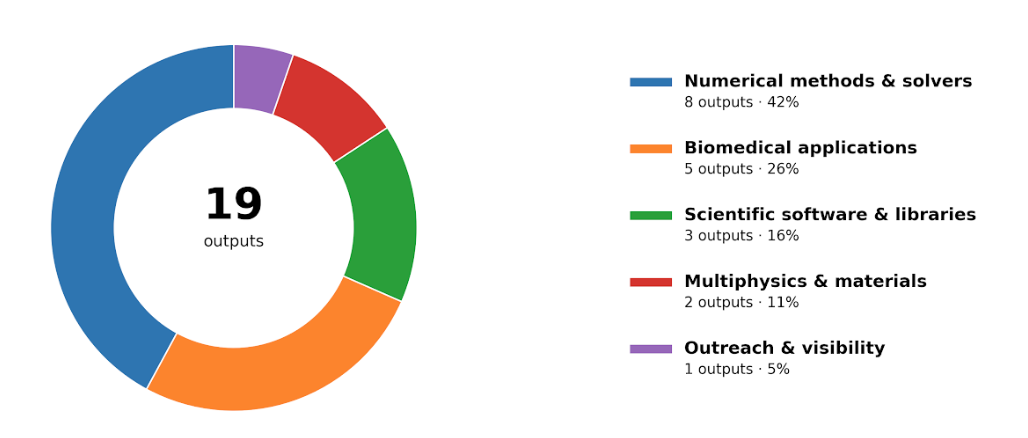
\includegraphics[width=\textwidth]{dissportfolio}
\caption{dealii-X Dissemination Portfolio.}\label{fig:dissportfolio}
\end{figure}


\subsubsection*{Article 17 of the Grant Agreement}

dealii-X project strictly follows the Article 17 of the Grant Agreement regarding communication, dissemination, promotion and visibility actions. In particular, all the dissemination results include both EU and EuroHPC logos and the following acknowledgment disclaimer: 


\noindent\emph{\small The European Union funded this study through the HORIZON-EUROHPC project ``dealii-X: an Exascale Framework for Digital Twins of the Human Body'' (topic HORIZON-EUROHPC-JU-2023-COE-03-01). Project Grant 101172493. Views and opinions expressed are, however, those of the author(s) only and do not necessarily reflect those of the European Union. Neither the European Union nor the granting authority can be held responsible for them.
}

As an example, Figure~\ref{fig:article17} displays the snapshot of the Article 17 implementation on the dealii-X webpage.

\begin{figure}[htbp]
\centering
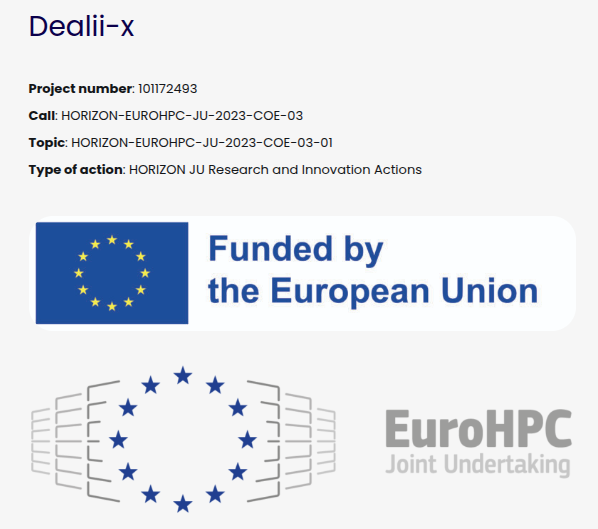
\includegraphics[width=0.5\textwidth]{article17}
\caption{Implementation of Article 17 on the dealii-X webpage. }\label{fig:article17}
\end{figure}

%\subsection{WP4.4: Stakeholder outreach and alignment with relevant EU initiatives and projects} 


\subsection{WP4.4: Stakeholder outreach and alignment with relevant EU initiatives and projects} \label{sec:wp4.4}



Outreach under this task is deliberately routed through the established networks of the
in silico medicine and HPC communities (see WP4.3) rather than through project-specific
channels, in order to maximize reach at limited cost. During the current reporting period
the emphasis has been on the professional stakeholder groups closest to the project's
technical results (clinical researchers, industry, HPC and modelling communities), while
engagement with patients, payers and policymakers remains at an early stage.


% Delete any row you cannot substantiate, and replace "planned" wording with concrete
% names/dates wherever you have them --- one named contact beats three generic promises.

\subsubsection*{Alignment with relevant EU initiatives and projects}

\begin{itemize}[left=1em, itemsep=0pt, topsep=0pt]
\item \textbf{EuroHPC JU ecosystem:} continuous alignment through CASTIEL2 (participation in the all-hands meeting, Tallinn), the HiDALGO2 clustering event, the joint minisymposium with EoCoE at SIAM PP 2026, and the CoE panel at HiPEAC 2026, ensuring exchange of good practice on exascale readiness and avoiding duplication of effort across Centres of Excellence.
\item \textbf{Virtual Human Twin initiative:} monitoring of and alignment with the VHT roadmap and the related EDITH/VHT infrastructure activities, mediated by the VPH Institute, to position the dealii-X solvers as computational components of the emerging European digital twin ecosystem.
% Add a concrete item if any partner attended a VHT/EDITH event or replied to a
% consultation --- this is the alignment reviewers will look for most closely..
\item \textbf{In silico medicine community:} alignment with the body of practice consolidated by previous EU-funded projects (In Silico World, STriTuVaD, MOBILISE-D, PRIMAGE, CompBioMed), in particular on model credibility and verification and validation reporting.
\end{itemize}

\subsubsection*{Follow-up on the intermediate review recommendations}

The Monitors of the intermediate project review identified stakeholder engagement and
exploitation as the weakest aspects of the project's planning and of the initial and
intermediate dissemination deliverables. The consortium accepts this assessment. The
activities reported above were designed primarily for the technical and scientific
communities and have not yet been translated into a systematic engagement process
covering the full range of stakeholders named in the Grant Agreement.

Work in the remaining period is therefore directed at converting the visibility already
achieved into genuine two-way engagement. The engagement approach is being reworked from
opportunistic dissemination towards a documented plan that identifies target organizations
for each stakeholder group and assigns responsibility for them within the consortium. The
structured instruments foreseen in the Grant Agreement --- focus groups, surveys and
semi-structured interviews --- will be applied first to the clinical and industrial
communities, which are closest to the project's results and where the consortium already
has established contacts. Engagement with patients, payers and policymakers will be
pursued through the intermediary organizations available to the consortium, in particular
the VPH Institute and the clinical partners' own networks, rather than through channels
the project would have to build from scratch in its final months. The outcome of these
activities, together with the corresponding indicators, will be reported in the final
dissemination deliverable.


\subsection{WP4.5: Exploitation}\label{sec:wp4.5}

Exploitation activities follow the tracking approach defined at the start of the task (M06),
based on a living register of exploitable results maintained jointly by all partners and
reviewed at the consortium all-hands meetings. The register distinguishes between
(i) open-source software results, exploited through the deal.II ecosystem and its user
community, (ii) methodological and performance results, exploited through scientific
publications and HPC access campaigns, and (iii) results with a direct industrial
exploitation path, exploited through integration into partner products and services. The
current status of the main exploitable results is summarized in
Table~\ref{tab:exploitation}.

\begin{table}[htbp]
\centering
\caption{Key exploitable results and their exploitation routes at M22.}\label{tab:exploitation}
\medskip
\renewcommand{\arraystretch}{1.2}
\footnotesize
\begin{tabular}{p{4cm}p{2.2cm}p{3.5cm}p{3.8cm}}
\toprule
\textbf{Exploitable result} & \textbf{Owner(s)} & \textbf{Route} & \textbf{Status at M22} \\
\midrule
Exascale-ready solver components (matrix-free kernels, multigrid, preconditioners) & Academic partners & Open source, upstream contribution to deal.II & Released and available to the deal.II user community \\
\midrule
Large-scale digital twin application codes & Application partners & Open source + use in partner research services & In development, staged releases \\
\midrule
Sparse direct solver technology & INPT, MUMPS & Transfer to MUMPS & Under discussion \\
\midrule
Low-code PoC platform & W1 and WP2 partners & Transfer to EXACT LAB and Dualistic & Under discussion \\
\midrule
Benchmarking and scalability results on EuroHPC systems & All partners & Publications, EuroHPC access proposals & Ongoing \\
\bottomrule
\end{tabular}
\end{table}
% Replace "Relevant partners"/"Under discussion" with the real owners and the actual
% stage once the claims discussion closes; and check the exact legal names of the
% receiving entities (MUMPS Technologies, exactlab s.r.l. and the second company you
% mentioned) before submission --- reviewers do check these.

\subsubsection*{Exploitation of technical results and HPC access}

\begin{itemize}[left=1em, itemsep=0pt, topsep=0pt]
\item \textbf{Open source first:} all core numerical developments are contributed upstream to the deal.II library and released under its open licence, which guarantees immediate availability to third parties, continuity beyond the project lifetime through an established maintainer community, and compliance with the Grant Agreement provisions on open science.
\item \textbf{HPC access campaigns:} the consortium has successfully obtained and used allocations on EuroHPC supercomputers, which have been exploited both for the scaling and performance campaigns reported in WP1--WP3 and as a demonstration of readiness of the dealii-X stack on European pre-exascale and exascale infrastructure.
% Insert: system names, call types (Extreme Scale / Regular / Benchmark), total core
% hours awarded and consumed. A single number here is the strongest exploitation
% evidence in the whole subsection.
\item \textbf{Uptake by third parties:} improvements contributed to deal.II benefit the wider user base of the library beyond the consortium, extending the reach of the project's results well past the biomedical application domain targeted by \mbox{dealii-X}.
% If you have download/clone statistics, releases containing dealii-X contributions,
% or external users/citations, add them here.
\item \textbf{Integration into partner software:} developed components are being integrated into the simulation workflows and toolchains maintained by the industrial and clinical partners, in line with the exploitation intentions declared in the Grant Agreement.
\end{itemize}

\subsubsection*{Sustainability beyond the project}

The intermediate review identified the sustainability of the project outcomes as an area
requiring strengthening. The consortium shares this assessment: while the exploitation of
technical results through open source and HPC campaigns is proceeding well, the
arrangements that will keep the dealii-X software stack maintained, supported and
commercially available after the end of the project were not yet defined at the time of the
review. 

Sustainability is therefore being addressed along three complementary lines, all of which
are under active discussion within the consortium.

Continuity of the core numerical developments is to a large extent already structural.
These are contributed upstream to \dealii{}, whose governance, release cycle and
contributor base are independent of dealii-X and predate it, so the exascale solver
components remain maintained, available and usable by third parties after the end of the
project without requiring any dedicated arrangement.

For those results whose long-term maintenance and commercial support depend on an
industrial actor, transfer routes towards partners of the consortium are being explored,
in particular for the sparse direct solver developments and for the low-code platform
together with its associated deployment and HPC integration know-how. These discussions
proceed in parallel with the clarification of ownership, access rights and exploitation
claims among the participating institutions, which is a precondition for any transfer
arrangement and is being conducted at coordinator level.

Finally, the consortium is preparing a set of publications documenting the results, the
performance achieved and the engineering experience gained in dealii-X, which will
consolidate the project's methodological legacy in the permanent scientific record
independently of the fate of any individual software component.

The outcome of all three lines will be consolidated in the final exploitation and
sustainability plan.

\newpage

\section{{Project Management (WP5)}}
\label{sec:wp5_management}

\subsection{Objectives}

WP5 is devoted to project management and administrative tasks. The main objective is to facilitate technical work, encourage synergy among partners, ensure consistency across tasks, and guarantee that expected results are achieved on time, of high quality, and compliant with the ethics requirements. Specifically, WP5 aims to:

\begin{itemize}[left=1em, itemsep=0pt, topsep=0pt]
\item Target- and result-oriented management of the project, including risk, conflict, and IP management.
\item Effective communication within the consortium and with the European Commission, ensuring deliverables and periodic reports are submitted on time.
\item Quality control of results and deliverables according to the defined procedures, ensuring internal review and approval prior to submission.
\end{itemize}

\subsection{WP5.1: Management}

\begin{itemize}[left=1em, itemsep=0pt, topsep=0pt]
	\item The management structure defined in D5.1 ``Project Management Handbook'' (M3, PM$^2$-based) remained stable and effective. The Project Management Board, chaired by the Project Coordinator, retains top-level authority; the Project Management Team handles day-to-day operations.
	\item Monthly consortium meetings continued without interruption, complemented by WP-level technical meetings and by the annual all-hands meeting held alongside the Research School ``Digital Twins of the Human Body'' (Trieste, December 2025).
	% Add the review date; adjust the cross-reference to point at your WP4.4/WP4.5
	% subsections if they carry their own labels.
	\item Decision-making, escalation and risk-monitoring procedures were applied as defined, and the internal documentation repository remains the single reference for minutes, deliverables and working documents.
	% Note here any changes in partner representatives or GA/CA amendments, if applicable.
\end{itemize}

\subsection{WP5.2: Communication}

\begin{itemize}[left=1em, itemsep=0pt, topsep=0pt]
	\item The Project Management Team continued to act as the interface between the consortium and the granting authority, preparing the periodic reporting (M12, M22) and the material for the intermediate review.
	\item Internal communication infrastructure (mailing lists, shared workspace, \texttt{[matrix]} instant messaging, project calendars) remained fully operational; details are given in Section~\ref{sec:wp4_communication}.
	\item Coordination between WP5 and WP4 was intensified in the second half of the reporting period, in particular on stakeholder engagement planning and on the preparation of the exploitation and sustainability arrangements.
\end{itemize}

\subsection{WP5.3: Quality Control}

\begin{itemize}[left=1em, itemsep=0pt, topsep=0pt]
	\item All formal deliverables submitted in the reporting period underwent internal review by assigned reviewers prior to submission, following the templates and procedures published on the internal workspace.
	\item Deliverables were submitted on schedule during this reporting period.
	% Check against the actual list; if anything slipped, name it, give the revised date
	% and state whether the EC approved it, as was done for D1.1 in the M12 report.
	\item The review procedure has been extended so that deliverables with a dissemination, stakeholder or exploitation component are additionally checked against the recommendations of the intermediate review before submission.
\end{itemize}

\subsection{Critical Risks and Mitigation}

\begin{itemize}[left=1em, itemsep=0pt, topsep=0pt]
	\item The risks identified during the RP1 --- delays in recruitment, technical dependencies between work packages, and the strategic work refocusing --- remained under control through monthly monitoring and early escalation. They are detailed in the Technical Report (part B) of the periodic reporting for RP1.
	\item The multigrid scalability limitation observed on JUPITER (Section~\ref{sec:wp1_dealii}) is being addressed with the support of the POP3 Centre of Excellence and by a dedicated task force established at RUB.
	\item Following the intermediate review, limited stakeholder engagement and the absence of a consolidated post-project sustainability arrangement are tracked as active issues rather than potential risks. Mitigation consists of the revised engagement activities reported under WP4.4 and the exploitation and technology transfer discussions reported under WP4.5, both monitored at the monthly consortium meetings.
	\item The main residual risk for the remaining period is the timely conclusion of the exploitation claims negotiated among the participating institutions concerning the conditions of the final exploitation and sustainability plan.
	\item The GPU-accelerated interface to PSCToolkit (WP1.4), originally due at M18, has been implemented and is awaiting submission to the \dealii{} main repository; the residual risk concerns the timing of the upstream review and of the subsequent large-scale evaluation, expected during Q3--Q4 2026. The AMG preconditioners themselves have already been validated at scale on MareNostrum 5 (Section~\ref{sec:wp1_psctoolkit}).
	\item Milestone \#13 (\emph{Upscale digital twins to pre-exascale environments}, M22) is only partially achieved (see Section~\ref{sec:wp2_applications}); the lung application requires further work on the surfactant boundary formulation before converged large-scale results can be produced. Progress is monitored at the monthly consortium meetings.
	
	
	% Add any technical residual risks from WP1--WP3 that management is tracking.
\end{itemize}

\subsection{Deliverable and milestone status}

\subsubsection*{Submitted deliverables}

The following deliverables have been submitted in M13-M22:
\begin{itemize}
	\item D4.5: Communication and Dissemination intermediate report (M15)
	\item D1.6: Tutorial based on external libraries (M17)
	\item D1.7: Report on \dealii{} improvements -- III semester (M17)
	\item D2.3: Report on applications improvements -- III semester (M17)
	\item D3.3: Integration of performance measuring tools (M17)
	\item D1.8: Polygonal Discretization in \dealii{} -- II (M22)
	\item D1.9: Report on \dealii{} improvements -- IV semester (M22)
	\item D2.4: Report on application improvements -- IV semester (M22)
	\item D2.7: Refined design of the PoC platform (M22)
	\item D3.4: Co-design and energe Efficiency report (M22)
	\item D5.3: Progress report M22 (M22)
\end{itemize}

Deliverables D1.6, D1.7, D2.3 and D3.3 have been accepted and approved by the RP1 by the Monitors during the RP1 project review. The Monitors requested changes to Deliverable D4.5 which will be implemented by September 2026 are resubmitted as described below.

\subsubsection*{Submitted deliverables}

The following milestone have been reached in M13-M22:
\begin{itemize}
	\item Milestone \#6: Parallel Polygonal Discretization Module (M14)
	\item Milestone \#7: Scalable Coupling Algorithms Framework Completion (M17)
	\item Milestone \#8: Cardiac Simulator Established for Exascale Computing (M17)
	\item Milestone \#9: Brain Simulator Established for Exascale Computing (M17)
	\item Milestone \#10: Multiscale Coupled Liver Model Completion (M17)
	\item Milestone \#11: Deployment of the First Version of the PoC Platform (M17)
	\item Milestone \#12: Polygonal GMG Module Completion (M22)
\end{itemize}

Milestones \#6-\#12 have been accepted and approved by the RP1 by the Monitors during the RP1 project review. 

\noindent\textbf{Status of Milestone \#13.}
Milestone \#13 (\emph{Upscale digital twins to pre-exascale environments}, M22) is partially achieved at the time of reporting. The brain and cardiac simulators have demonstrated large-scale runs on pre-exascale systems, while the lung application requires further work on the surfactant boundary formulation before converged large-scale results can be produced, and the liver application is scaling up network complexity towards full-organ geometries. Completion is expected M24, and progress is being closely monitored.


\subsection{Reporting Period RP1 review}

The intermediate project review for the reporting period RP1 was held on 13 May 2026, and the formal review report was received on 2 July 2026. The Monitors acknowledged the technical progress of the project and recommended strengthening the stakeholder engagement and exploitation activities; these recommendations have been taken up by the consortium and are reflected in Sections~\ref{sec:wp4.4} and~\ref{sec:wp4.5}, and in the present section. The requested changes to Deliverables D1.3, D4.4 and D4.5 are being prepared and will be submitted by September 2026.


\subsection{Clarification on travel costs}

The Monitors observed that the travel budget appears overestimated for some partners. The partner INPT reports travel costs exceeding 15\% of its personnel costs in RP1, while remaining within the overall frame of the action at that partner. These costs correspond to trips, detailed in the Financial Statement of INPT, made by members of the MUMPS development team who are closely involved in dealii-X although not directly funded by the project. In particular, they attended the project meeting in Trieste, where the synchronisation between partners necessary to deliver the content of WP1.5 took place, and which also supported several other dealii-X activities. In addition, results achieved by the INPT team, including results obtained by members not directly funded by dealii-X, were presented at SIAM PP in Berlin, aligning the project's activities with the scientific community.


\subsection{Gender balance}

The intermediate review noted that gender balance was not addressed in the documents
submitted for the first reporting period. The consortium reports the following situation at
M22. Of the 13 researchers fully funded by the project across the beneficiaries, 3 are
women. At the level of scientific leadership, 3 of the 13 principal investigators of the
consortium are women, as are 1 of the 4 work package leaders. Recruitment for project positions followed the applicable EU and institutional guidelines, with vacancies advertised through open international calls. The consortium notes that, for the specific technical profiles required by some partners, recruitment proved challenging regardless of the gender of applicants.

The consortium is aware that these figures reflect a wider structural imbalance in the
field, and the project partners seek to contribute to addressing it through open recruitment practices and by
giving early-career researchers a visible role in the project's training and dissemination
activities.

Following the Monitors' suggestion, the consortium has begun examining whether the organ
simulation models could incorporate sex- or gender-specific parameters. The patient-specific
simulators are driven by subject-derived imaging data and therefore already reflect
individual anatomy, whereas the material parameters currently in use are not differentiated
by sex. Whether such a differentiation is feasible within the remaining project time, and
for which applications, is being assessed together with the application partners in WP2;
the outcome will be reported in the final application deliverables.

\label{MyLastPage}

\end{document}
